\section{Модели спиновых систем}
\subsection{Однородная цепочка спинов}
% фтористый апатит (mrjs-2019) x2 

% \begin{figure}
%   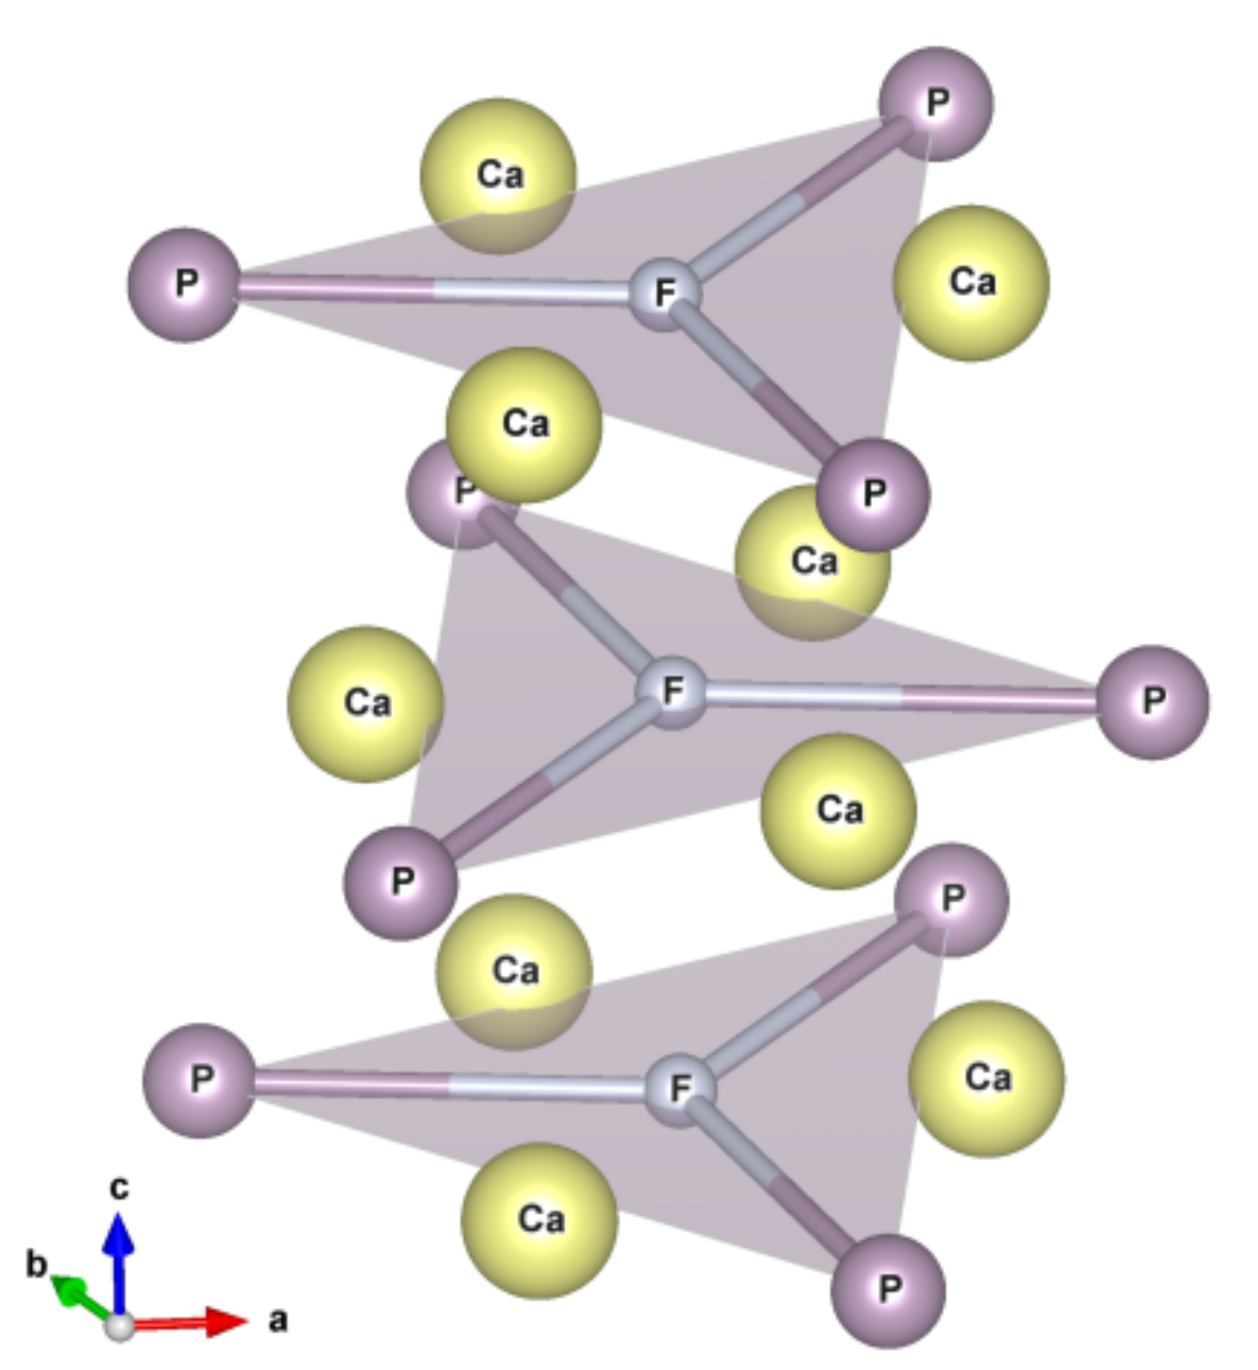
\includegraphics[width=\textwidth]{model-uniform-chain-fluorapatite-structure.png}
%   \caption{.
%   Часть кристаллической структуры Фтористй апатит Ca$_{10}$(PO$_4$)$_6$F$_2$, показывающая окружение атомов фтора. 
% Атомы кислорода были удалены для ясности. 
% Атомы фтора равномерно разнесены ($r_{FF}= 3.44$\AA) и расположены в колонны вдоль $c$-оси кристалла. 
% Каждый атом фтора окружен тремя равноудаленными атомами фосфора при $r_{FP} = 3.67$\AA, 
% которые расположены в вершинах равносторонних треугольников на плоскости, перпендикулярной к $c$-оси, 
% а также тремя ионами Ca\textrm{II} на расстоянии $2.34$\AA.
%   }
% \end{figure}



% \subsubsection{декогеренция (JETP-2018) (JMR-2019)}

\subsection{Зигзагобразная цепочка спинов}
% гамбергит (JMR-2020) G.A. Bochkin and et al., \textit{J. Magn. Res.} \textbf{319}, 106816, (2020)


% \begin{figure}
%   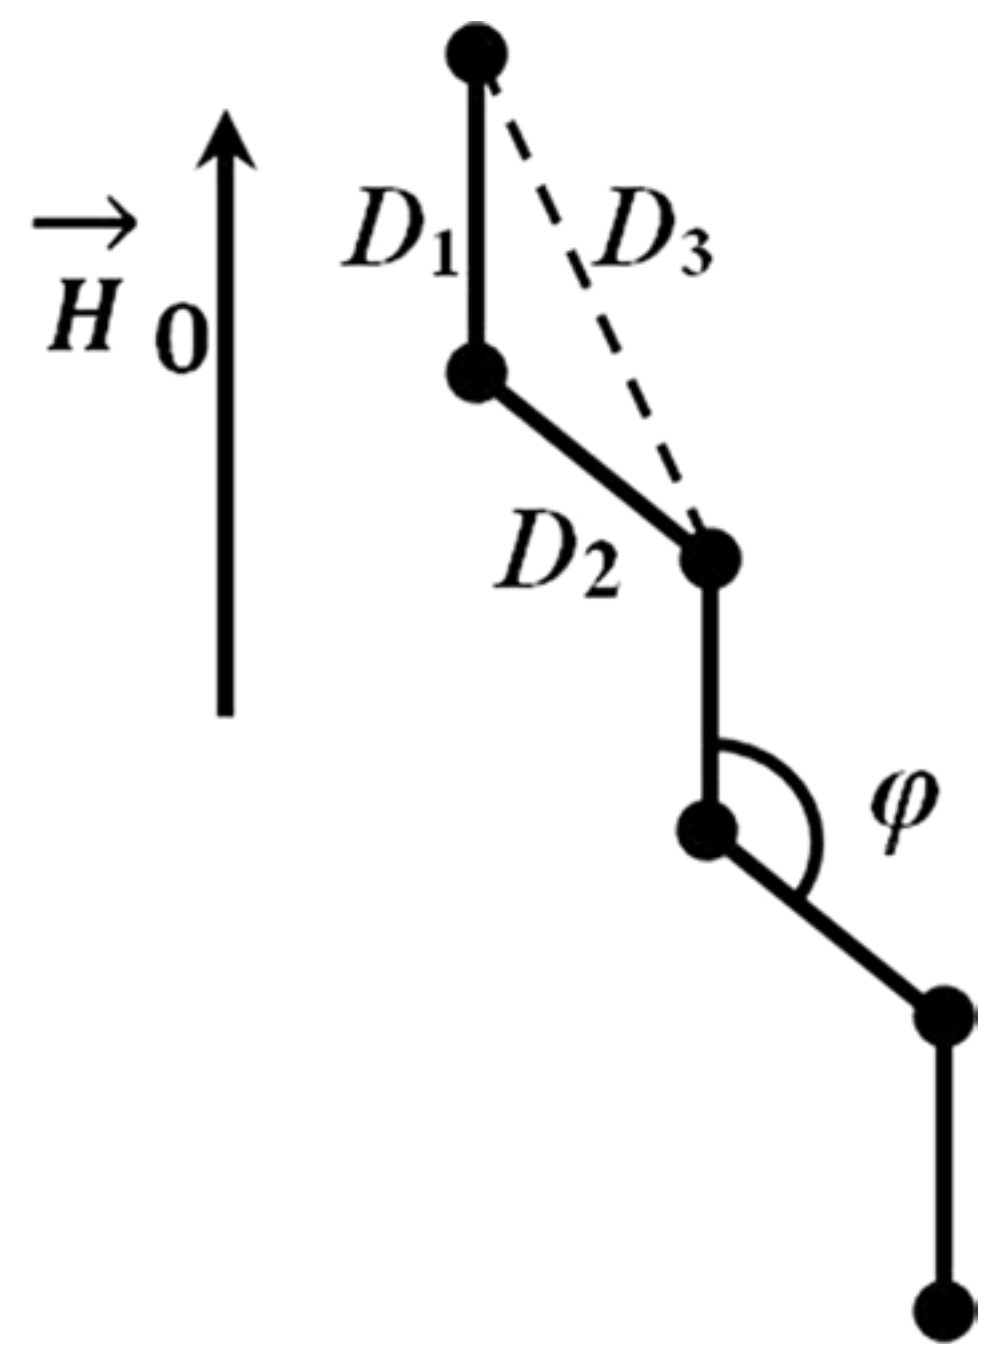
\includegraphics[width=0.5\textwidth]{model-zigzag-chain-schema.png}
%   \caption{Схема зигзагообзаной цепочки}
% \end{figure}
% 
%     Константы взаимодействия
%         $$D_1=\dfrac{\gamma^2\hbar }{r^3}, $$
%         $$D_2 = D_1\dfrac{ 3\cos^2 \varphi -1 }{2} $$
%         $$D_3 = D_1 \dfrac{ 3\sin^2 \frac{\varphi}{2} -1}{16 \sin^3, \frac{\varphi}{2}}$$
%         где $\gamma$ - гиромагнитное отношение,
%         $\varphi$ - угол между соседними связями,
%         $r$ - расстояние между соседними спинами в цепочке.
% 
%     Базовый случай это когда одна линия связи направлена вдоль поля. тогда констаты будет самой большой в доль поля.
%     Изменяя угол к полю мы можем получить как альтернированную цепочку так и однородную.
%     В приближении ближайших и следующих соседей, задача решается аналитически, но она
%     не дает полной картины. Поэтому мы решали данную систему численно.
% 
%     \begin{figure}
%       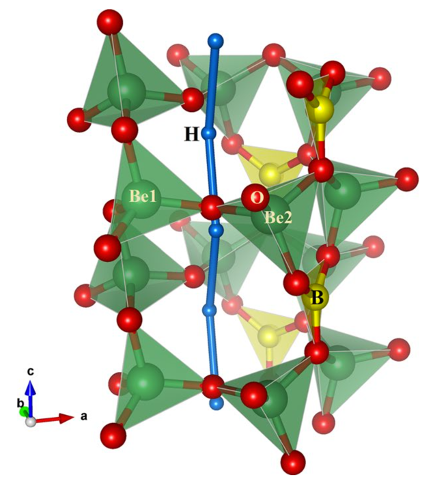
\includegraphics[width=0.85\textwidth]{model-zigzag-chain-hambergite-structure.png}
%       \caption{Hанопора со спин-несущих молекулами во внешнем сильном магнитном поле $\vec B$}
%     \end{figure}
% 
%     Гамбергит $Be_2BO_3(OH)$ 
%         \begin{itemize}
%             \item Дипольное взаимодействия между ближайшими спинами протонов в цепи в 17 раз сильнее, чем со спинами окружающих цепей (в худшем случае).
%             \item Взаимодействия с остальными окружающими спинами по меньшей мере в 30 раз слабее.
%             \item Вклад дипольной связи между спинами в одной и той же цепи доминирует над остальными взаимодействиями.
%         \end{itemize}
% 
%     В одномерных цепочках возникают когерентности только $\pm 2$ порядка
%     и следовательно дисперсия распределения будет небольшой
%     и мы не увидим запутанных кластеров.
%     Однако в альтернированная цепочке гамбергита возникают когерентности $\pm 4$ порядка
%     и следовательно можно использовать эту модель для исследования многочастичной запутанности.
%     The distance to these two protons is 4.49 Å
%     The distance between a given chain and surrounding proton chains is at least 2.1 times larger than the distance between neighbors in the chain.
% 


\subsection{Модель эквивалентных спинов}
% , нанопора 
%   \begin{figure}
%     \begin{subfigure}[t]{0.32\textwidth}
%       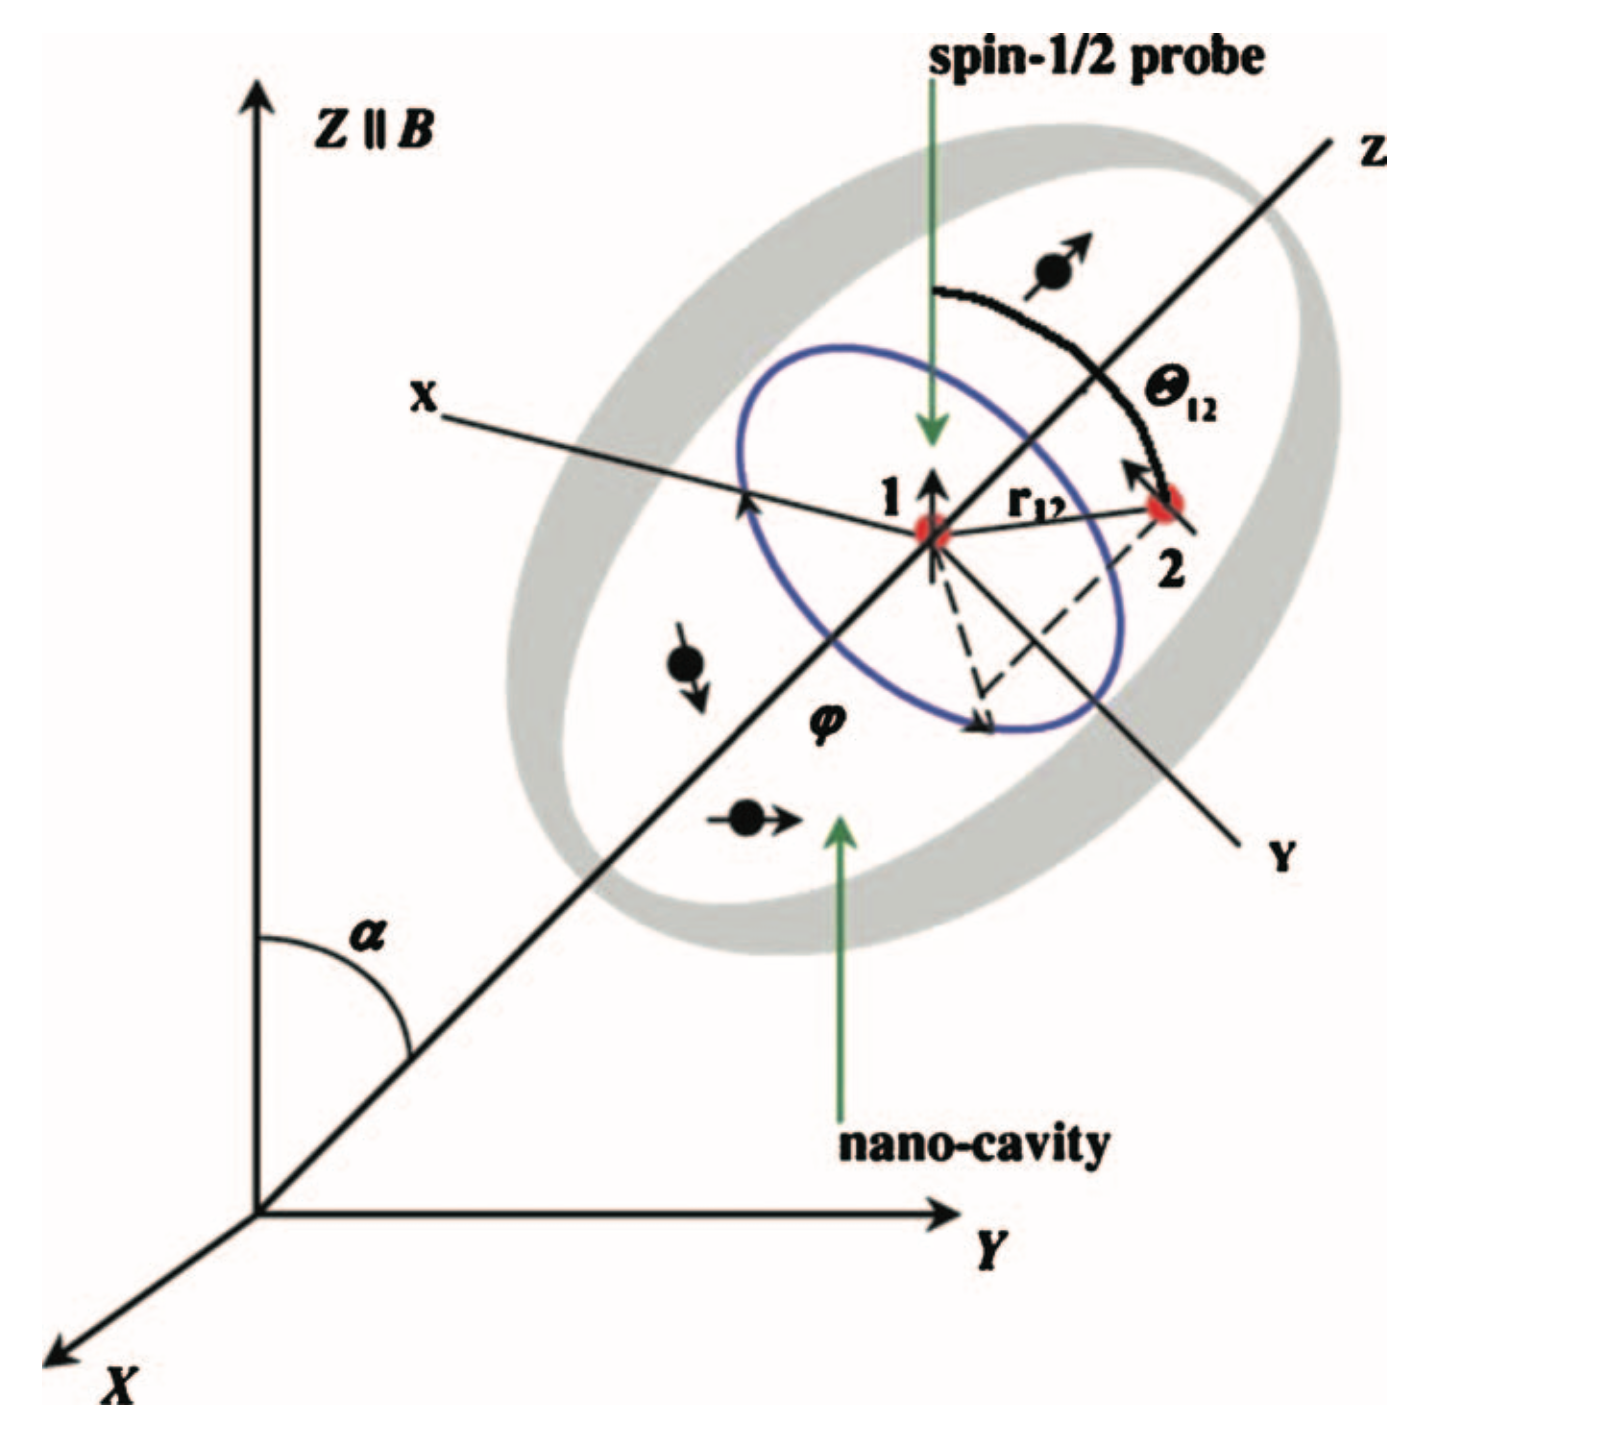
\includegraphics[width=\textwidth]{model-nanopore-schema.png}
%       \caption{
%         Hанопора\cite{Baugh2001} 
%         со спин-несущих молекулами во внешнем сильном магнитном поле $\vec B$.
%       }
%     \end{subfigure}
%     \hfill
%     \begin{subfigure}[t]{0.32\textwidth}
%       \includegraphics[width=0.8\textwidth]{model-nanopore-nmr-spectrum.png}
%       \caption{
%         Молекулярная диффузия газа быстрее флип-флоп процессов.
%         Вся система характеризуется одной константой $D$.
%       }
%     \end{subfigure}
%     \hfill
%     \begin{subfigure}[t]{0.32\textwidth}
%       \includegraphics[width=\textwidth]{model-nanopore-film.png}
%       \caption{
%         Значение константы связи $D$ зависит как от газа, 
%         так и от эффективного давления в нанопоре ($\approx 1$ кБар)
%       }
%     \end{subfigure}
%     \captionsetup{skip=-0.1mm}
%     \caption{}
%   \end{figure}
% 
%  % J. Baugh, A. Kleinhammes, D. Han, Q. Wang, and Y. Wu, Science 294, 1505 (2001).
%  
%  Так как молекулярная диффузия газа быстрее флип-флоп процессов,
%  вся система характеризуется одной константой взаимодейсвия $D$.
%  Значение константы связи $D$ зависит как от газа, так и от эффективного давления в нанопоре ($\approx 1$ кБар).
%   
%  Hydrogenated amorphous silicon (Гидрогенизированный аморфный кремний) 
%  
%  Для исследования многочастичной запутанности нам нужна модель,
%  в которой почти все частицы взаимодействуют друг с другом,
%  а также она должна поддаваться счету.
%  Мы решили рассмотреть модель эквивалентных спинов.
%  Такой модели соотвествует нанопора заполеннея спин несущими частицами.
% 
%  Такие нанопоры получаются выдавлием под давлением ~ 1 кБар  на специальной подложке.
% 
%  Необходимо подчеркнуть, что существуют некоторые ограничения для реализации описанной модели при исследовании нанопористых соединений с МК - ЯМР-методами. Например, модель предполагает, что все нанопоры имеют одинаковый объем и одинаковую "несферическую" форму.
% 
%  Молекулярная диффузия газа очень быстрая в сравнениидиподьных флип флом процессов
%  Каждая частица успевает обойти всю нанопору пока пройдет флипфлоп
%  Поэтому можно описать взаимодействие с одной константой
% 
%  Среднняя константа связи зависит как от газа, так и от эффективного давления в нанопоре
% 
%  При низких температурах диффузия побеждает?
%  Какие частицы?
